\documentclass[times, utf8, seminar]{fer}
\usepackage{booktabs}

\begin{document}

% TODO: Navedite naslov rada.
\title{Stohastičko modeliranje u financijama}

% TODO: Navedite vaše ime i prezime.
\author{Ivan Almer}

% TODO: Navedite ime i prezime mentora.
\voditelj{Tomislav Burić}

\maketitle

\tableofcontents

\chapter{Uvod}
Naivno je misliti da se tržište uglavnom ponaša po nekom skupu pravila i da je moguće predvidjeti kretanja s apsolutnom preciznošću. To bi značilo da postoji „besplatan ručak“ i da možemo uvišestručiti naša sredstva bez imalo rizika. Naravno da nitko od nas nije prvi koji se sjetio povećati svoj kapital brzo i efikasno, ali naravno da to ne dolazi bez određene opasnosti da ćemo izgubiti svoj kapital.

Tržište je mjesto sa izuzetno puno igrača gdje svaki igrač želi zaradu i naravno da nitko ne želi gubiti. Kada netko gubi novac, druga ga strana dobiva, ali za svakog igrača u toj velikoj igri gubici su neizbježni. Cilj je što manje puta izvući deblji kraj i što manje biti na gubitničkoj strani.

Svatko može naslijepo uložiti dio svog kapitala u neki financijski instrument i nadati se da će baš na taj način zaraditi, no malo je vjerojatno da će takav potez donijeti puno dobroga. Sigurno postoje i neki bolji načini kako da analiziramo i kvantificiramo kvalitetu naših ulagačkih ideja s ciljem maksimizacije profita. Budući da se tržište ponaša prilično nedeterministički jasno nam je da to neće biti lak zadatak. Upravo s tom idejom dolazimo to toga da se i u naše modele uvede već spomenuti nedeterminizam s određenim karakteristikama i da na taj način pokušamo naučiti promatrati naizgled kaotično ponašanje tržišta.

Stohastički procesi imaju široku primjenu u financijama. Od modeliranja cijena dionica, kamatnih stopa, do određivanja cijena nekih financijskih derivata i procjene rizika ulaganja. Stohastičko modeliranje je oblik financijskog modeliranja koji se koristi za pomoć u donošenju odluka o ulaganju. Takvim pristupom možemo dobiti podatke i predvidjeti moguće ishode s mjerom nepredvidivosti ili slučajnosti. Mnoge firme koriste stohastičko modeliranje da bi optimizirale svoje portfelje i upravljale svojom imovinom. Jedan je od primjera stohastičkog modeliranja, na primjer, Monte Carlo simulacija, kojom se može modelirati ponašanje portfelja temeljeno na razdiobi povrata individualnih dionica.

Svrha ovog seminarskog rada je napraviti pregled i pobliže objasniti načine uporabe stohastičkog modeliranja u financijama. Iza većine modela stoje neke pretpostavke o ponašanju pojava koje promatramo, koje mogu biti opravdane, ali ponekad se ne obraća puno pažnje na te pretpostavke i model se primjenjuje kada to uistinu ne bi trebalo. U tom svjetlu, ovim radom također želim istaknuti i važnost pretpostavki modela i metoda koje će biti opisane.

\chapter{Black-Scholes Model}

Jedan od najpoznatijih modela za određivanje cijena opcija je Black-Scholes model za koji su znanstvenici osvojili Nobelovu nagradu za ekonomiju. Danas se smatra jednim od najboljih načina za određivanje „fer“ cijene opcija, jer bi u protivnom postojala mogućnost arbitraže.

Black-Scholes model ima pretpostavku na distribuciju cijene dionice da ona mora biti log-normalna, što ima smisla jer cijene dionica ne mogu biti negativne. Razlog za korištenje upravo te distribucije je taj da se cijena dionica vrlo često ponaša kao desno nakrivljena distribucija sa nešto debljim repovima.

\begin{figure}[h!]
\centering
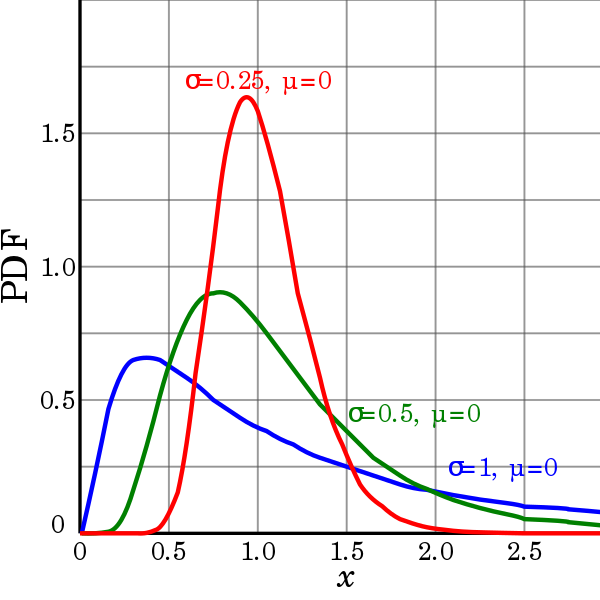
\includegraphics[scale=0.4]{img/log_normal_pdf.png}
\caption{Funkcija gustoće vjerojatnosti log-normalne razdiobe}
\label{fig:log_normal_pdf}
\end{figure}

\noindent Ostale pretpostavke uključuju:
\begin{itemize}
    \item[\textbullet] Opcija je europska (ne može se iskoristiti prije dospijeća)
    \item[\textbullet] Kamatna stopa nerizičnog ulaganja i volatilnost su konstantni
    \item[\textbullet] Dionica ne isplaćuje dividende
    \item[\textbullet] Kretanje tržišta se ne može predvidjeti
\end{itemize}

Izvod ovog modela je mjesto gdje se događaju najzanimljivije stvari i gdje se zapravo najbolje vidi moć stohastičkih procesa. Prvi korak u izvodu je korištenje Itove leme na funkciju cijene opcije za koju vrijedi pretpostavka da ovisi o vremenu i cijeni dionice.

Cijena dionice je modelirana geometrijskim Brownovim gibanjem, a za neki stohastički proces kažemo da ima geometrijsko Brownovo gibanje, ako zadovoljava diferencijalnu jednadžbu:

\begin{centering}
    $dS_t = \mu S_t dt + \sigma S_t dW_t$ \\
\end{centering}

\noindent gdje je $W_t$ Brownovo gibanje definirano kao:
\begin{enumerate}
    \item $W_0 = 0$
    \item $W$ ima nezavisne priraste za svaki $t > 0$
    \item $W_{t+u} - W_t \sim N(0, u)$
    \item $W_t$ je kontinuirano u vremenu
\end{enumerate}

\section{Call i Put opcije}
Opcija je oblik financijskog derivata, koji kupcu ugovora daje pravo, ali ne i obavezu, da pri isteku ugovora (dospijeću) kupi ili proda neko sredstvo po unaprijed dogovorenoj cijeni. Dvije su vrste opcija - call i put. Call opcija kupcu ugovora daje pravo da pri dospijeću kupi sredstvo (npr. dionicu) po cijeni dogovorenoj pri kupnji ugovora. Put opcija se ponaša obrnuto, odnosno kupcu ugovora daje pravo da pri dospijeću proda određeno sredstvo po unaprijed dogovorenoj cijeni. Svaki takav ugovor karakteriziran je sljedećim parametrima:
\begin{itemize}
    \item[\textbullet] cijena ugovora
    \item[\textbullet] dospijeće (vrijeme isteka ugovora)
    \item[\textbullet] izvršna cijena
\end{itemize}

\noindent Primjer uporabe opcija:

Pretpostavimo da možemo trgovati dionicom \textbf{XYZ} kojoj je trenutna cijena $S_0 = 100$. U ovom trenutku mi smo uvjereni da će cijena dionice u budućnosti rasti i kao alternativu direktne kupovine dionice, odlučili smo kupiti call opciju za tu dionicu. Recimo da se $1$ call opcija, izvršne cijene $K = 102$ i dospijeća od jednog mjeseca, prodaje po cijeni $C = 6$, a budući da je jedan ugovor call opcije obično ne odnose na $1$ dionicu nego na njih $100$, onda je cijena jednog takvog ugovora $100 * 6 = 600$. Nakon mjesec dana pogledajmo sljedeća $2$ scenarija:
\begin{itemize}
    \item[\textbullet] cijena dionice se ponaša u skladu s našim očekivanjem i porasla je na $S_t = 120$
    \item[\textbullet] cijena dionice je pala i sada iznosi $S_t = 90$
\end{itemize}
\noindent U drugom slučaju naš ugovor postaje bezvrijedan i gubimo naš uloženi kapital (odnosno naš profit je $-600$). Međutim, u slučaju da se ostvari prvi scenarij možemo iskoristiti pravo da kupimo $100$ dionica po cijeni od $102$. Budući da se te dionice trenutno prodaju po cijeni $120$, nakon što ih kupimo po cijeni od $102$ prodamo ih po tržišnoj cijeni i ostvarili smo profit od $(120 - 102) * 100 - 600 = 1200$.

\section{Pregled formule}

\[ C = N(d_1)S_0 - N(d_2)Ke^{-rt} \]
\[ gdje \hspace{0.1cm} je \hspace{0.2cm} d_1 = \frac{ln\frac{S_t}{K} + (r+\frac{\sigma^2}{2})t}{\sigma\sqrt{t}} \]
\[i \hspace{0.2cm} d_2 = d_1 - \sigma \sqrt{t}\]

\noindent $C =$ cijena Call opcije \\
$N =$ funkcija razdiobe normalne razdiobe\\
$S_0 =$ trenutna cijena dionice (spot price)\\
$K =$ izvršna cijena dionice (strike price)\\
$r =$ kamatna stopa nerizičnog ulaganja\\
$t =$ vrijeme do dospijeća\\
$\sigma =$ volatilnost cijene dionice \\

\noindent Kada imamo sve gore navedene parametre, formulom dobijemo cijenu europske call opcije. Cijena put opcije iste dionice, s istim dospijećem i istom izvršnom cijenom dobije se pomoću put-call pariteta koji povezuje te dvije cijene:

    \[ C + PV(K) = P + S_0 \]
    \[ PV(K) = \frac{K}{(1+r)^t} \]

\noindent $C =$ cijena Call opcije \\
$P =$ cijena Put opcije \\
$PV(K) =$ izvršna cijena diskontirana na današnji dan (PV - present value)\\
$S_0 =$ trenutna cijena dionice (spot price)\\
$r =$ kamatna stopa nerizičnog ulaganja \\

Kada postoji odstupanje od Put-Call pariteta, odnosno 2 strane jednadžbe nisu jednake, onda postoji prilika za arbitražu. Međutim takve prilike su obično jako rijetke i kratkog vijeka, a ako se i nađu, onda su potrebne izuzetno velike količine kapitala ne bi li se ostvario značajan profit.

% INSERT - prica o odredivanju implied volatilitya iz call - put opcija

\chapter{Simulacije i financijski modeli}

% INSERT - opcenito o simulacijama
\section{Monte-Carlo metoda}
Monte-Carlo simulacija je metoda generiranja slučajnih varijabli u svrhu modeliranja rizika odnosno nesigurnosti nekog sustava. Slučajne varijable su modelirane po nekim poznatim distribucijama i svaka simulacija generira drugačije rezultate, jer je Monte-Carlo metoda nedeterministička. Simulacija se pokreće puno puta (npr. 1 000 000) i ako nas zanima npr. najgorih 1\% ishoda onda imamo 10 000 takvih ishoda i možemo vidjeti koliko loše stvari mogu poći.

\subsection{Var (Value at Risk)}
Jedna od primjena MC simulacija je kod odredivanje VaR-a (value at risk). To je metoda razvijena od strane velike banke JP Morgan za predviđanje najgoreg očekivanog povrata nekog portfelja uz određeni interval povjerenja. Točnije, ta metoda odgovara na pitanje: "S nekom fiksiranom sigurnošću (npr. 99\%) koliko ću najviše kapitala izgubiti u nekom određenom periodu?", a odgovor je oblika "U zadanom periodu, na temelju danih podataka, sa sigurnošću od 99\% možemo tvrditi da gubitak kapitala neće biti veći od $X$"

% Monte Carlo za VaR za 1 varijablu - primjer

% Matematika iza MC simulacije za multi-asset portfolio
Konkretnije, za portfelj koji sadrži više dionica moguće je velikim brojem Monte-Carlo simulacija dobiti

\section{Primjeri simulacije na BS modelu}

\chapter{Modeli za mjerenje kreditnog rizika}
Kreditni rizik je rizik propasti (defaulta) kompanije i smisleno je da osobe koje izdaju kredite žele primati premiju na rizik koji preuzimaju davanjem novaca drugoj strani. Što je kompanija stabilnija, rizik defaulta je manji, pa time očekujemo i da kamatna stopa kredita, koji je kompanija željela podići, bude manja.

\section{Strukturni modeli}
Ovakvi se modeli oslanjaju na određivanje rizika iz vrijednosti firme. Jedan od takvih modela je Mertonov model. Pretpostavka je da se vrijednost firme kreće kao geometrijsko Brownovo gibanje, kao što je i bio slučaj kod Black-Scholesove formule gdje se cijena dionice modelirala kao geometrijsko Brownovo gibanje.
Zanimljivo je to da se ovim modelom zapravo modelira call opcija za vrijednost cijele kompanije uzimajući u obzir i sva dugovanja koje kompanija ima i na taj se način evaluira rizik.

% insert formula
%[Prodiskutirati formulu…]
%[proučiti I dati primjer interpretacije modela]

\section{Modeli intenziteta}
% [potencijalno izbaciti ovaj dio ovisno o kolicini ovoga ispod]
% [opis I navesti primjene]


\chapter{Stohastička teorija portfelja (STP)}
Stohastička teorija portfelja je relativno nova matematička teorija za analizu tržišta dionica, koju je razvio E. Robert Fernholz 2002. godine. STP oslanja se na uprabu kontinuiranih slučajnih procesa (preciznije neprekidnih semi-martingala) za predstavljanje cijena financijskih instrumenata.

Svaka dionica u portfelju predstavljena je kao proces njene cijene, obično u logaritamskom obliku. Neka imamo $n$ dionica u našem portfelju, onda je cijena dionice $i$ za $i=1,...,n$ dana kontinuiranim semi-martingalom:

\[ d \log X(t) = \gamma(y)dt + \sum_{\nu=1}^{d}\xi_{\nu}(t)dW_{\nu}(t) \]

gdje je $(W_1,...,W_n)$ Brownovo gibanje, $\gamma$ je takozvana mjera rasta (\textit{eng. growth rate}) i zadovoljava \(\int_{0}^{T} |\gamma(t)| \,dt < \infty\). \(\xi_{\nu}, \nu = 1,...,n\) je proces volatilnosti (\textit{eng. volatility process}) i on predstavlja osjetljivost \(X\) na \(\nu\)-ti izvor nesigurnosti (\textit{eng. source of uncertainty}).
Za sve \(\xi_{\nu}, \nu = 1,...,n\) vrijedi sljedeće:

\[ \int_{0}^{T} (\xi_1(t) + \cdots + \xi_n(t)) \,dt < \infty\]
\[ \lim_{t\to\infty} t^{-1}(\xi_1^2(t) + \cdots + \xi_n^2(t))\log\log t = 0 \]
\[ \xi_1^2(t) + \cdots + \xi_n^2(t) > 0 \]



Na prethodno opisani način definirano je ponašanje jedne dionice i bitno je spomenuti da se ovdje uzima kao pretpostavka da postoji samo 1 dionica na tržištu, odnosno \(X(t)\) predstavlja cjelokupnu tržišnu vrijednost firme u trenutku $t$.
Pretpostavimo sada da imamo cijelu familiju dionica \(X_i,\) \(i = 1,...,n\) koje  se ponašaju na ovaj način:

\[ d \log X_i(t) = \gamma_i(y)dt + \sum_{\nu=1}^{d}\xi_{i\nu}(t)dW_{\nu}(t) \]

% bolje objasniti ksi, odnosno osjetljivost na src of uncertainty
% 1.1.12 u knjizi mozda je zanimljivo za pokazati?
% optimizacija portfelja, moda se VaR koristi kao heuristika
% pokazati hedging sa opcijama (^ ali to gore pokazati)

\chapter{Zaključak}
Zaključak.

\bibliography{literatura}
\bibliographystyle{fer}

\chapter{Sažetak}
Sažetak.

\end{document}
